
\documentclass[10pt,sigconf,screen,authorversion,review,anonymous]{acmart}

%% \BibTeX command to typeset BibTeX logo in the docs
\AtBeginDocument{%
  \providecommand\BibTeX{{%
    \normalfont B\kern-0.5em{\scshape i\kern-0.25em b}\kern-0.8em\TeX}}}

%% Rights management information
\setcopyright{acmcopyright}
\copyrightyear{2018}
\acmYear{2018}
\acmDOI{XXXXXXX.XXXXXXX}

%% Commands for a proceedings abstract or paper
\acmConference[Conference acronym 'XX]{Make sure to enter the correct
  conference title from your rights confirmation emai}{June 03--05,
  2018}{Woodstock, NY}
% \acmBooktitle{Woodstock '18: ACM Symposium on Neural Gaze Detection,
%  June 03--05, 2018, Woodstock, NY} 
\acmPrice{15.00}
\acmISBN{978-1-4503-XXXX-X/18/06}

%% Submission ID
%%\acmSubmissionID{123-A56-BU3}

%% For managing citations
%%\citestyle{acmauthoryear}

%% Extra invaluable commands
\usepackage{subcaption}
\usepackage{booktabs}
\usepackage{multirow}
\usepackage{cases}
\usepackage{empheq}
\usepackage{xfrac}
% \usepackage{float}
\usepackage{cleveref}

\graphicspath{{figure/}{figures/}}
\DeclareMathOperator*{\argmin}{argmin}
\DeclareMathOperator{\sech}{sech}
\newcommand{\tabhead}[1]{{\bfseries#1}}




%% End of the preamble
\begin{document}


%% Title
\title[A short title]{The Name of the Title is Hope}


%% Authors
\author{Ben Trovato}
\authornote{Both authors contributed equally to this research.}
\email{trovato@corporation.com}
\orcid{1234-5678-9012}
\author{G.K.M. Tobin}
\authornotemark[1]
\email{webmaster@marysville-ohio.com}
\affiliation{%
  \institution{Institute for Clarity in Documentation}
  \streetaddress{P.O. Box 1212}
  \city{Dublin}
  \state{Ohio}
  \country{USA}
  \postcode{43017-6221}
}

\author{Lars Th{\o}rv{\"a}ld}
\affiliation{%
  \institution{The Th{\o}rv{\"a}ld Group}
  \streetaddress{1 Th{\o}rv{\"a}ld Circle}
  \city{Hekla}
  \country{Iceland}}
\email{larst@affiliation.org}

\author{Valerie B\'eranger}
\affiliation{%
  \institution{Inria Paris-Rocquencourt}
  \city{Rocquencourt}
  \country{France}
}

%% Short authors in page headers
\renewcommand{\shortauthors}{Trovato and Tobin, et al.}


%% Abstract
\begin{abstract}
  This is stripped-down \LaTeX\ tamplate for documents following the ACM format. The teaser figure is a big win. And normal references can be added like \cite{Abril07} and software version like \cite{delebecque:hal-02090402-condensed}
\end{abstract}


%% Computing Classification System from http://dl.acm.org/ccs.cfm
\begin{CCSXML}
<ccs2012>
   <concept>
       <concept_id>10010405.10010432</concept_id>
       <concept_desc>Applied computing~Physical sciences and engineering</concept_desc>
       <concept_significance>500</concept_significance>
       </concept>
 </ccs2012>
\end{CCSXML}

\ccsdesc[500]{Applied computing~Physical sciences and engineering}

%% Keywords
\keywords{datasets, neural networks, gaze detection, text tagging}

%% A "teaser" image
\begin{teaserfigure}
  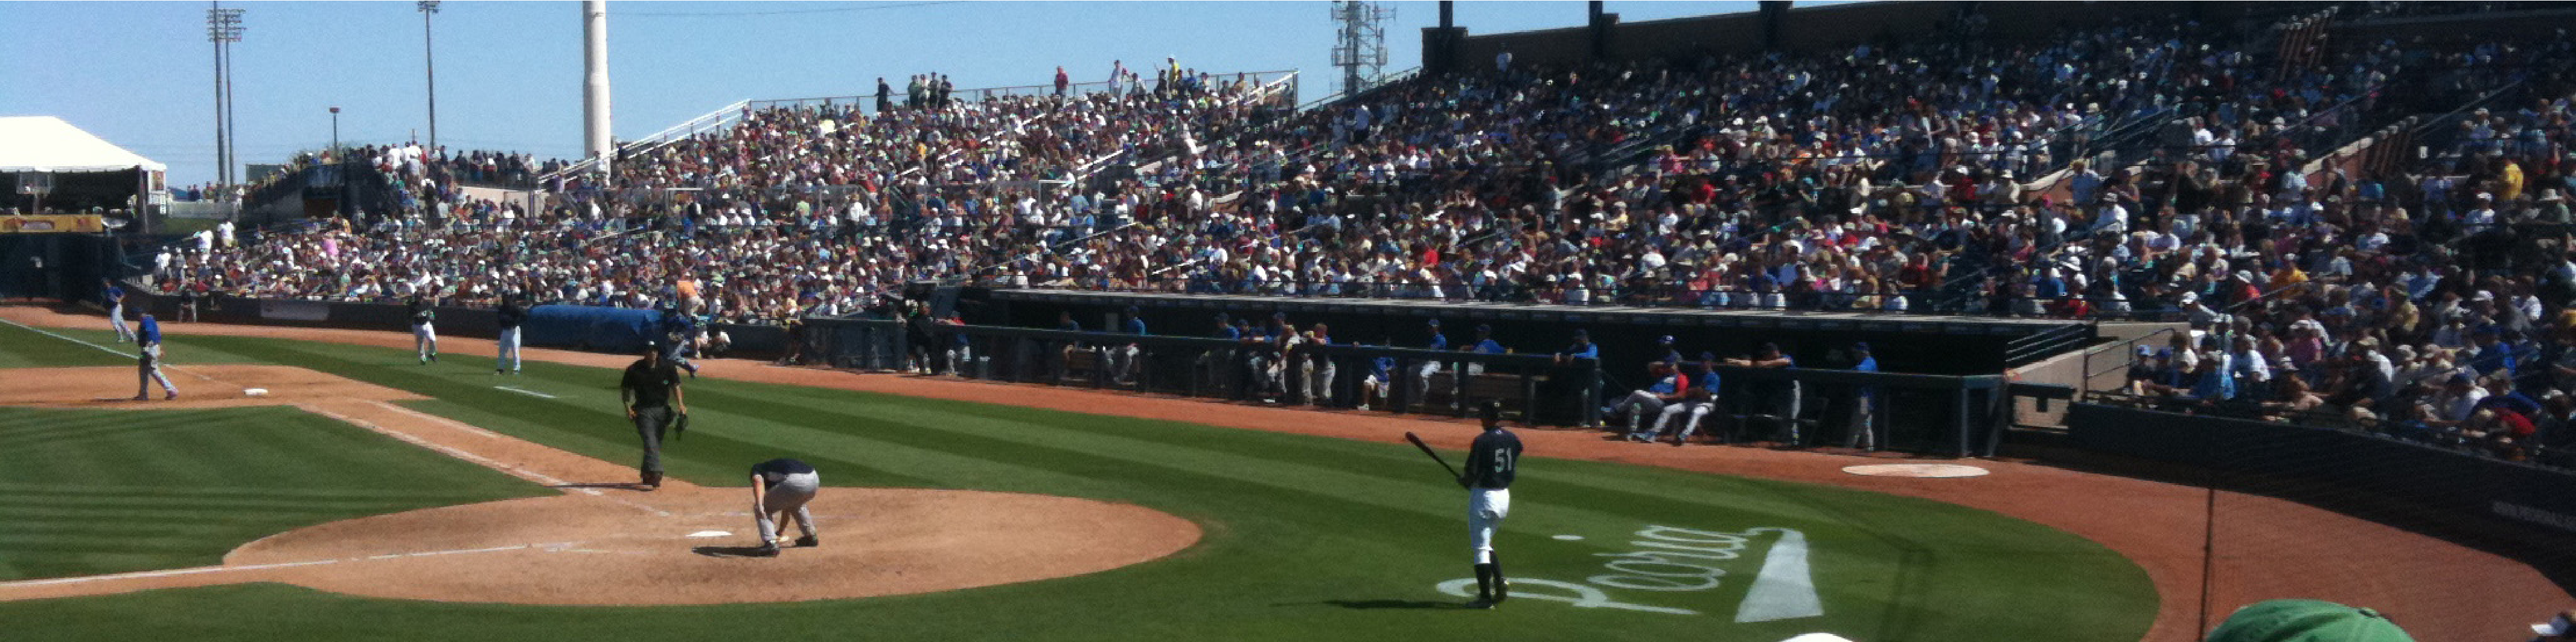
\includegraphics[width=\textwidth]{sampleteaser}
  \caption{Seattle Mariners at Spring Training, 2010.}
  \Description{Enjoying the baseball game from the third-base
  seats. Ichiro Suzuki preparing to bat.}
  \label{fig:teaser}
\end{teaserfigure}

\received{20 February 2007}
\received[revised]{12 March 2009}
\received[accepted]{5 June 2009}


%% Processes and builds the above
\maketitle

%% Main sections
\section{Introduction}
\label{sec.intro}
\section{Methods}
\label{sec.method}

\section{Results}
\label{sec.results}
\section{Discussion}
\label{sec.discusion}
\section{Future work}
\label{sec.conclusion}


%% Acknowledgments
\begin{acks}
To Robert, for the bagels and explaining CMYK and color spaces.
\end{acks}


%% Bibliography style
\bibliographystyle{bibformats/acmdefault}
\bibliography{references}


%% Appendix
\appendix




\end{document}
